\section{Auswertung}

Die mittlere freie Weglänge $\overline{w}$ und den Dampfdruck $p_\text{sät}$, der bei den verschiedenen
Messreihen vorlag lässt sich mithilfe der Gleichung \ref{eq:5} bestimmen. Die Daten
sind in Tabelle \ref{tab:1} dargestellt.

\begin{table}
  \centering
  \caption{Die mittleren freien Weglängen und die Dampfdrücke von Hg bei verschiedenen
  Temperaturen.}
  \label{tab:1}
  \begin{tabular}{c c c}
    \toprule
    $T \, / \, K$ & $\overline{w} \, / \, cm$ & $p_\text{sät} \, / \, mbar$ \\
    \midrule
    298,55 & $\num{5.30e-1}$ & $\num{5.47e-3}$ \\
    377,15 & $\num{4.36e-3}$ & $\num{6.60e-1}$ \\
    418,65 & $\num{7.16e-4}$ & $\num{4.05}$    \\
    465,15 & $\num{1.37e-4}$ & $\num{20.92}$ \\
    \bottomrule
  \end{tabular}
\end{table}

\subsection{Differentielle Energieverteilung}

Nun soll aus den in den Abbildungen \ref{abb:} und \ref{abb:} gemessenen Kurven
die differentielle Energieverteilung bestimmt werden. Dazu wird die Steigung
an verschiedenen Stellen gemessen und gegen die Bremsspannung $U_a$ aufgetragen.
Die gemessenen Steigungen von der ersten Messreihe, die bei $T = \SI{25.4}{\degree\celsius}$
durchgeführt wurde, sind in Tabelle \ref{tab:2} dargestellt.

\begin{table}[H]
  \centering
  \caption{Darstellung der Steigungen a in Abhängigkeit von der Bremsspannung $U_a$
  der ersten Messreihe.}
  \label{tab:2}
  \begin{tabular}{c c}
    \toprule
    $U_a \, / \, V$ & $a$
    \midrule
    0,40 & 0 \\
    0,80 & 0 \\
    1,20 & 0 \\
    1,60 & 0 \\
    2,00 & 0 \\
    2,60 & 0,033  \\
    4,00 & 0,025  \\
    5,20 & 0,050  \\
    5,80 & 0,100  \\
    6,24 & 0,083  \\
    6,72 & 0,083  \\
    7,12 & 0,083  \\
    7,68 & 0,110  \\
    8,00 & 0,125  \\
    8,22 & 0,200  \\
    8,42 & 0,200  \\
    8,62 & 0,200  \\
    8,82 & 0,200  \\
    9,00 & 0,250  \\
    9,16 & 0,250  \\
    9,38 & 0,286  \\
    9,64 & 0,330   \\
    9,84 & 0,500    \\
    \bottomrule
  \end{tabular}
\end{table}

Mit diesen Messwerten ergibt sich nun der Graph, welcher in Abbildung \ref{abb:3}
dargestellt ist.

\begin{figure}[H]
  \centering
  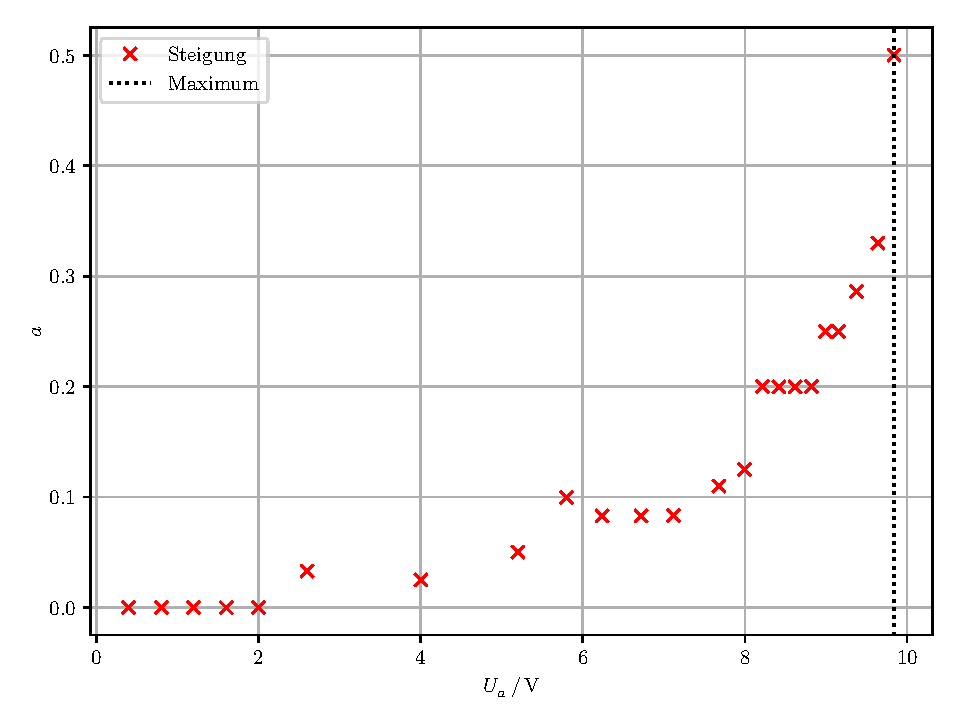
\includegraphics[width=\textwidth]{plot1.pdf}
  \caption{Graphische Darstellung der differentiellen Energieverteilung bei $T = \SI{25.4}{\degree\celsius}$.}
  \label{abb:3}
\end{figure}

Da die Elektronen mit einer Spanunng von \SI{11}{\volt} beschleunigt werden lässt
sich aus dem Graphen das Kontaktpotential K der Apparatur berechnen, welches in diesem
Fall $ K = \SI{1.16}{\volt}$ ist.

Die zweite Messreiche wird bei $ T = \SI{145.5}{\degree\celsius}$ durchgeführt.
Aufgrund der höheren Temperatur sind die bestimmten Werte auch anders als bei der
ersten Messreihe. Die berechneten Steigungen sind in Tabelle \ref{tab:2} dargestellt
und auch in diesem Fall werden die differentiellen Energieverteilungen gegen
die Bremsspannung in Abbildung \ref{abb:4} dargestellt.

\begin{table}[H]
  \centering
  \caption{Darstellung der Steigungen a in Abhängigkeit von der Bremsspannung $U_a$
  der zweiten Messreihe.}
  \label{tab:2}
  \begin{tabular}{c c}
    \toprule
    $U_a \, / \, V$ & $a$
    \midrule
    0,08 & 0,750  \\
    0,28 & 0,830  \\
    0,54 & 0,714  \\
    0,86 & 0,667  \\
    1,24 & 0,750  \\
    1,66 & 0,462  \\
    2,12 & 0,300  \\
    2,60 & 0,100  \\
    3,00 & 0,100  \\
    3,40 & 0,200  \\
    3,80 & 0,200  \\
    4,20 & 0,200  \\
    4,60 & 0,200  \\
    5,00 & 0,300  \\
    5,40 & 0,100  \\
    5,80 & 0,100  \\
    6,20 & 0,100  \\
    6,60 & 0,100  \\
    7,20 & 0,050  \\
    8,00 & 0  \\
    8,40 & 0  \\
    8,60 & 0  \\
    \bottomrule
  \end{tabular}
\end{table}

\begin{figure}[H]
  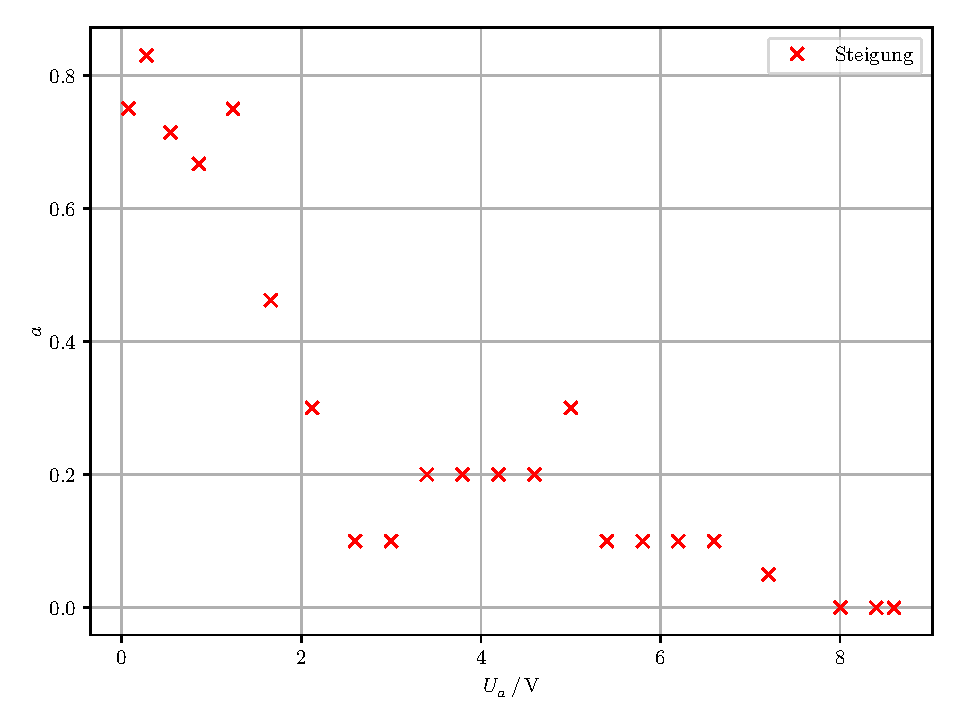
\includegraphics[width=\textwidth]{plot2.pdf}
  \caption{Graphische Darstellung der differentiellen Energieverteilung bei $T = \SI{145.5}{\degree\celsius}$.}
  \label{abb:4}
\end{figure}

Die Form der Messwerte der zweiten Messreihe unterscheidet sich so stark von der
ersten, weil bei der höheren Temperatur die mittlere freie Weglänge viel geringer ist
und die Elektronen mit einer höheren Wahrscheinlichkeit mit den Hg-Atomen wechselwirken.

\subsection{Franck-Hertz-Kurve}
